\chapter{Thermal design}
\label{ch:thermal}

\section{The thermal chain}

Heat leaves the die through three resistances in series:

\begin{equation}
  \Tj = T_\mathrm{liq}
      + P_\mathrm{tot}\,\Rthha
      + \frac{P_\mathrm{tot}}{6}\left(\Rthcs + \Rthjc\right),
  \label{eq:thermal-chain}
\end{equation}

\noindent where $\Rthha$ is the cold plate to coolant resistance carrying the
total loss, and $\Rthcs$ (the insulating pad) and $\Rthjc$ (junction to case)
each carry one device's share.

\begin{figure}[htbp]
\centering
% Catena termica dell'eq. (thermal-chain): ogni dispositivo ha i suoi R_jc e R_cs, il
% dissipatore e' comune. Le perdite sono generatori di corrente, le temperature potenziali.
\begin{circuitikz}[font=\footnotesize]
  \draw (0,0) node[ground]{} to[I, l={$P_k$}] (0,2)
        to[short, -*] (0.6,2) node[below=2pt]{$T_{j,k}$}
        to[R, l={$\Rthjc$}, -*] (3.0,2) node[below=2pt]{$T_{c,k}$}
        to[R, l={$\Rthcs$, pad}, -*] (5.4,2) node[below right=1pt]{$T_\mathrm{hs}$}
        to[R, l={$\Rthha$}] (9.6,2)
        to[V, l={$T_\mathrm{liq}$}, invert] (9.6,0) node[ground]{};
  % gli altri cinque dispositivi arrivano sullo stesso nodo
  \draw[dashed] (5.4,2) -- (5.4,3.0) -- (3.4,3.0);
  \node[anchor=east, font=\scriptsize] at (3.4,3.0) {five more branches $P$--$\Rthjc$--$\Rthcs$};
  \node[font=\scriptsize, align=center, text width=62mm] at (5.0,0.55)
       {$\Rthha$: one value for the ideal plate; spreading, conduction and convection in the real rail (\cref{sec:cooling})};
\end{circuitikz}

\caption{\Cref{eq:thermal-chain} as a network: losses are current sources,
temperatures potentials. Each device has its own path through the case and
the pad; all six meet at the heat sink.}
\label{fig:thermalnet}
\end{figure}

\begin{table}[htbp]
\centering
\caption{Thermal chain at the design point.}
\label{tab:thermal-chain}
\begin{tabular}{llrr}
\toprule
Node & Resistance & Value & Temperature \\
\midrule
Coolant   & ---      & ---                              & \SI{65.00}{\celsius} \\
Cold plate & $\Rthha$ & \SI{0.01}{\celsius\per\watt}     & \SI{66.28}{\celsius} \\
Case      & $\Rthcs$ & \SI{0.50}{\celsius\per\watt}     & \SI{76.96}{\celsius} \\
Junction  & $\Rthjc$ & \SI{0.22864}{\celsius\per\watt}  & \textbf{\SI{81.84}{\celsius}} \\
\midrule
\multicolumn{3}{l}{Limit} & \SI{150}{\celsius} \\
\multicolumn{3}{l}{\textbf{Margin}} & \textbf{\SI{68.16}{\celsius}} \\
\bottomrule
\end{tabular}
\end{table}

The junction-to-case value is not an assumption: it is the sum of the Cauer
network contained in the vendor thermal description
($0.024544 + 0.077043 + 0.040982 + 0.086066 =
\SI{0.22864}{\celsius\per\watt}$), and it coincides with the typical
datasheet figure of \SI{0.23}{\celsius\per\watt}~\cite{wolfspeed_e3m0016}.
The datasheet maximum is \SI{0.31}{\celsius\per\watt}; at the rated point
the difference is \SI{1.7}{\celsius}, at locked rotor \SI{5}{\celsius}:
exactly the part of the \SI{30}{\celsius} allowance of criterion C1 that
\cref{tab:criteria} leaves unallocated. A worst-case die is covered, with
nothing left over.

\subsection{Equal loss distribution}

\Cref{eq:thermal-chain} divides the total loss by six. The assumption is
exact here by symmetry: the three phases are identical up to a
\SI{120}{\degree} shift, and within one leg the high-side and low-side
devices exchange roles every half fundamental period. It fails at very low
output frequency, where the current dwells, and in the limit of zero
frequency it fails completely: that case is treated on its own in
\cref{sec:lockedrotor}.

\section{The loop between losses and temperature}

Losses depend on temperature and temperature depends on losses, so the
operating point is the fixed point of \cref{eq:thermal-chain} and not the
result of a single evaluation. The sweep of the pad resistance below gives
the slope directly, as the change of loss over the change of junction
temperature between its end points:
%
\begin{equation}
  \frac{\mathrm{d}P_\mathrm{tot}}{\mathrm{d}\Tj} = \SI{0.392}{\watt\per\celsius},
\end{equation}
%
and hence a loop gain
%
\begin{equation}
  G = \frac{\mathrm{d}P_\mathrm{tot}}{\mathrm{d}\Tj}
      \left(\Rthha + \frac{\Rthcs + \Rthjc}{6}\right) = 0.052 ,
  \qquad \frac{1}{1-G} = 1.054 .
\end{equation}

The loop converges comfortably and amplifies by only \SI{5}{\percent},
half as much as with the \SI{40}{\milli\ohm} device of the first iterations
($G = 0.107$). The reason is the new loss split: conduction, which is the
temperature-dependent part through $\Rdson$, is now \SI{45}{\percent} of
the total instead of \SI{85}{\percent}. The solution is still obtained by
iterating the simulation until the assumed and resulting case temperatures
agree, which takes three or four passes.

\section{The insulating pad dominates}
\label{sec:rthcs}

\begin{finding}{The dominant unknown is the cheapest part of the chain}
Of the \SI{16.8}{\celsius} rise from coolant to junction, the insulating pad
accounts for \SI{10.7}{\celsius} and the junction-to-case path for
\SI{4.9}{\celsius}. The single most influential parameter in the thermal
design is therefore a piece of ceramic worth a few cents, whose thermal
resistance depends on its thickness, its area, and the torque with which the
device is bolted down. With the \SI{16}{\milli\ohm} device the pad weighs
even more than before: its \SI{0.5}{\celsius\per\watt} is more than twice
the $\Rthjc$ of the die.

It was also, initially, entirely absent from the model: the simulation
implicitly assumed the TO-247 was soldered to the cold plate. On the device
of the first iterations, correcting it moved the junction temperature from
\SI{79.5}{} to \SI{95.3}{\celsius}.
\end{finding}

Because $\Rthcs$ is an assumption rather than a measurement, the design is
verified across the whole plausible range, from a high-performance ceramic
pad to a mediocre silicone one.

\begin{figure}[htbp]
\centering
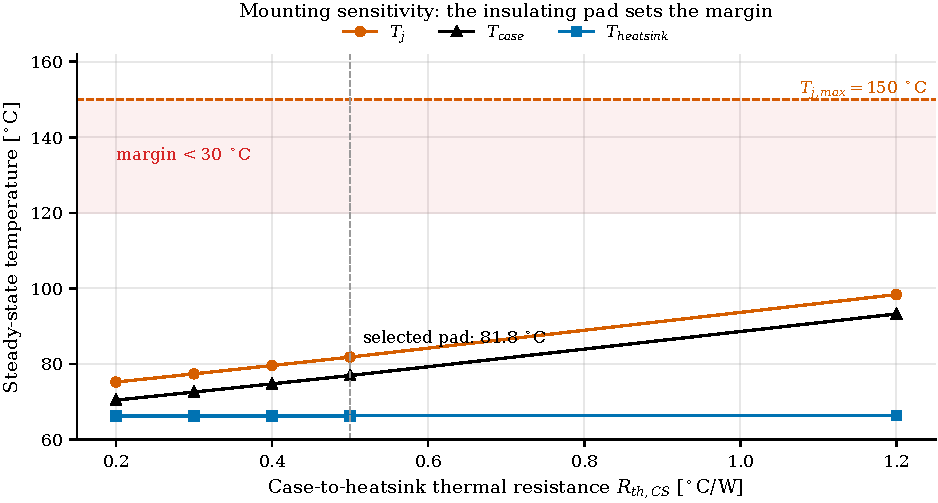
\includegraphics[width=\textwidth]{plecs_12_sensibilita_r_th_cs.pdf}
\caption{Junction, case and cold-plate temperatures against the pad thermal
resistance at the rated point, with the \SI{150}{\celsius} limit and the band
in which the margin falls below \SI{30}{\celsius}.}
\label{fig:rthcs}
\end{figure}

\begin{table}[htbp]
\centering
\caption{Sensitivity to the insulating pad at the rated point. Each row is a
separate solution of the loss--temperature loop, not an extrapolation of the
first.}
\label{tab:rthcs}
\begin{tabular}{lrrrr}
\toprule
$\Rthcs$ & $P_\mathrm{tot}$ & $\Tcase$ & $\Tj$ & Margin \\
\midrule
\SI{0.20}{\celsius\per\watt} & \SI{125.53}{\watt} & \SI{70.44}{\celsius} & \SI{75.22}{\celsius} & \SI{74.78}{\celsius} \\
\SI{0.30}{\celsius\per\watt} & \SI{126.35}{\watt} & \SI{72.58}{\celsius} & \SI{77.40}{\celsius} & \SI{72.60}{\celsius} \\
\SI{0.40}{\celsius\per\watt} & \SI{127.22}{\watt} & \SI{74.75}{\celsius} & \SI{79.60}{\celsius} & \SI{70.40}{\celsius} \\
\textbf{\SI{0.50}{\celsius\per\watt}} & \textbf{\SI{128.09}{\watt}} & \textbf{\SI{76.96}{\celsius}} & \textbf{\SI{81.84}{\celsius}} & \textbf{\SI{68.16}{\celsius}} \\
\SI{1.20}{\celsius\per\watt} & \SI{134.61}{\watt} & \SI{93.27}{\celsius} & \SI{98.40}{\celsius} & \SI{51.60}{\celsius} \\
\bottomrule
\end{tabular}
\end{table}

At the rated point the pad hardly matters: even the worst silicone pad
leaves \SI{51.6}{\celsius} of margin. The locked rotor bounds the pad. There, one device carries almost
three times the rated-point loss per device, and every tenth of a
\si{\celsius\per\watt} costs about \SI{7}{\celsius}
(\cref{sec:lockedrotor}). C1 is met up to
$\Rthcs = \SI{0.62}{\celsius\per\watt}$ with the coolant at
\SI{65}{\celsius}.

A ceramic pad (alumina or aluminium nitride) is therefore selected, with
\SI{0.50}{\celsius\per\watt} taken as a prudent class value and
\SI{0.62}{\celsius\per\watt} written into the mounting specification as
the value not to be exceeded, torque included. A filled silicone pad, at
\SI{0.5}{}--\SI{1.2}{\celsius\per\watt}, is no longer acceptable: it would
pass the rated point and fail the stalled motor. Mounting without
insulation is not an option, because the tab of the TO-247 is the drain and
would put \SI{800}{\volt} on a chassis-referenced cold plate.

The ideal plate overstates what a real rail does, and \cref{sec:cooling}
replaces it: on the rail as drawn, C1 holds only up to
\SI{0.50}{\celsius\per\watt}, which becomes the mounting limit, and the
pad adopted is aluminium nitride with a phase-change interface material, at
a design value of \SI{0.18}{\celsius\per\watt}.

\section{Locked rotor}
\label{sec:lockedrotor}

At zero output frequency the symmetry of \cref{eq:thermal-chain} is gone.
The modulator holds the phase angle at which phase~1 is at its peak: phase~1
carries the full \SI{42.4}{\ampere} as direct current, phases 2 and 3 carry
\SI{-21.2}{\ampere} each. In phase~1 the high-side device is the active
switch: it conducts for \SI{53}{\percent} of each switching period and
hard-switches \SI{42.4}{\ampere} at \SI{20}{\kilo\hertz}, while the
low-side device conducts the remaining time as a synchronous rectifier and
switches at nearly zero voltage. That
high-side device is the hottest in the converter, and it is the one C1 is
written for.

The case is simulated on the same model, with the output frequency set to
zero and the modulation amplitude re-trimmed until the phase current is
\SI{42.4}{\ampere} (\SI{26.8}{\volt} are enough, since a stalled machine
presents only its stator resistance). The thermal boundary is applied per
device: the hottest device sees the common cold plate, heated by the total
loss, plus its \emph{own} loss through the pad, not the average.

\begin{table}[htbp]
\centering
\caption{Locked rotor on the final design ($R_g = \SI{5}{}/\SI{12.5}{\ohm}$,
dead time \SI{260}{\nano\second}, $\Rthcs = \SI{0.5}{\celsius\per\watt}$),
hottest device.}
\label{tab:lockedrotor}
\begin{tabular}{lrr}
\toprule
Coolant & \SI{65}{\celsius} & \SI{70}{\celsius} \\
\midrule
Phase current (DC)          & \SI{42.43}{\ampere} & \SI{42.43}{\ampere} \\
Loss, hottest device        & \SI{61.25}{\watt}  & \SI{62.29}{\watt} \\
Loss, converter             & \SI{140.97}{\watt} & \SI{143.17}{\watt} \\
Case temperature            & \SI{97.04}{\celsius} & \SI{102.58}{\celsius} \\
\textbf{Junction temperature} & \textbf{\SI{111.05}{\celsius}} & \textbf{\SI{116.82}{\celsius}} \\
Margin to C1 (\SI{120}{\celsius}) & \SI{8.95}{\celsius} & \SI{3.18}{\celsius} \\
Margin to the \SI{150}{\celsius} limit & \SI{38.95}{\celsius} & \SI{33.18}{\celsius} \\
\bottomrule
\end{tabular}
\end{table}

The hottest device dissipates \SI{61.3}{\watt}, 2.9 times its share at the
rated point, while the converter as a whole dissipates only
\SI{10}{\percent} more. The loss is concentrated in one device, and a better
cold plate alone cannot fix that, because the heat has to cross the pad and
the die of a single device. The cold plate is at \SI{66.4}{\celsius}; the
\SI{45}{\celsius} between it and the junction are spent entirely in
$\Rthcs$ and $\Rthjc$.

Three sensitivities complete the picture:
%
\begin{itemize}
  \item Coolant temperature: \SI{+5}{\celsius} at the inlet gives
        \SI{+5.8}{\celsius} at the junction: slightly more than one to one,
        through the loop gain. C1 holds at \SI{70}{\celsius} with
        \SI{3.2}{\celsius} to spare (\cref{app:assumptions}, A.9).
  \item Pad: from \SI{0.5}{} to \SI{0.6}{} and
        \SI{0.7}{\celsius\per\watt} the junction rises to \SI{118.3}{} and
        \SI{125.8}{\celsius}; C1 is lost beyond
        \SI{0.62}{\celsius\per\watt}.
  \item Turn-off gate resistance: raising it from \SI{12.5}{} to
        \SI{15}{\ohm}, which a longer loop than \SI{20}{\nano\henry} would
        demand, costs \SI{2.0}{\celsius} (computed on the previous model
        version, with \SI{160}{\nano\second} of dead time; at \SI{12.5}{\ohm}
        the two versions agree within \SI{0.1}{\celsius}).
\end{itemize}

The die and the pad settle in well under a second; the cold plate needs
tens of seconds, but its share of the rise is only \SI{1.4}{\celsius}.
Holding a vehicle on a slope lasts longer than the former, so the steady
state is the correct criterion, and a conservative one.

\subsection{Where the loss of the hottest device comes from}
\label{sec:lrdpwm}

Splitting the \SI{61.25}{\watt} of the hottest device, by running the same
case with conduction and switching losses enabled one at a time, gives
\SI{21.2}{\watt} of conduction and \SI{40.0}{\watt} of switching. At locked
rotor, as at the rated point, switching dominates: the device hard-switches
\SI{42.4}{\ampere} twenty thousand times a second through the
\SI{12.5}{\ohm} that C2 imposes. The opposite device of the same leg
conducts for the rest of the period and carries only \SI{18.4}{\watt}.

That split is what makes discontinuous modulation interesting here, and
also what limits it. Clamping phase~1 to the positive rail (DPWM-MAX) stops
its switching, but it does not remove the current: the high-side device now
conducts for the whole period instead of \SI{53}{\percent} of it.

\begin{table}[htbp]
\centering
\caption{Locked rotor with three zero sequences, coolant \SI{65}{\celsius},
$\Rthcs = \SI{0.5}{\celsius\per\watt}$, same model and thermal loop as
\cref{tab:lockedrotor}; hottest device A1 in all three. DPWM-MAX clamps
phase~1 to the positive rail, DPWM-MIN phases 2 and 3 to the negative one.
The clamp is verified by the switching loss of the clamped device, zero.}
\label{tab:lrdpwm}
\small
\begin{tabular}{lrrrrr}
\toprule
Zero sequence & Conduction & Switching & Total & $\Tj$ & Converter \\
\midrule
\textbf{SVPWM (adopted)} & \SI{21.2}{\watt} & \SI{40.0}{\watt} & \SI{61.3}{\watt} & \textbf{\SI{111.1}{\celsius}} & \SI{141.0}{\watt} \\
DPWM-MAX & \SI{38.3}{\watt} & 0 & \SI{38.3}{\watt} & \textbf{\SI{93.9}{\celsius}} & \SI{96.0}{\watt} \\
DPWM-MIN & \SI{1.5}{\watt} & \SI{38.6}{\watt} & \SI{40.1}{\watt} & \SI{95.2}{\celsius} & \SI{95.9}{\watt} \\
\bottomrule
\end{tabular}
\end{table}

DPWM-MAX lowers the hottest junction by \SI{17.2}{\celsius}, to
\SI{93.9}{\celsius}, and the converter loss by a third. It is less than
removing the \SI{40}{\watt} of switching would suggest, because
\SI{17}{\watt} of conduction move onto the same device: the net saving on
it is \SI{23}{\watt}, not \SI{40}{\watt}. DPWM-MIN clamps the other two
phases instead; phase~1 keeps switching at a duty of \SI{5}{\percent}, and
the two devices of its leg end at \SI{95.2}{} and \SI{92.9}{\celsius}. It
is nearly as good, and either would serve. How this margin is used, as a
recommendation to the controller and not as a basis for sizing, is stated in
\cref{tab:sysassume}.

\begin{finding}{Discontinuous modulation would not have saved the \SI{40}{\milli\ohm} device}
If modulation could have kept the first device inside C1, the device change
was avoidable. The same three cases, run on the \SI{40}{\milli\ohm} devices
at their datasheet gate resistance of \SI{2.5}{\ohm}, show that it could
not:
%
\begin{center}
\small
\begin{tabular}{lrrrr}
\toprule
 & SVPWM & DPWM-MAX & DPWM-MIN & Best offset$^\ast$ \\
\midrule
C3M0040120K & \SI{140.8}{\celsius} & \SI{192.0}{\celsius} & \SI{176.2}{\celsius} & \SI{125.4}{\celsius} \\
E3M0040120K & \SI{142.3}{\celsius} & \SI{190.7}{\celsius} & \SI{174.4}{\celsius} & \SI{125.3}{\celsius} \\
\bottomrule
\multicolumn{5}{l}{\footnotesize $^\ast$ common-mode offset that balances the two devices of the leg ($d_1 \approx 0.41$).}
\end{tabular}
\end{center}
%
Where conduction dominates, as it does with \SI{40}{\milli\ohm} (\SI{61}{}
of \SI{77}{\watt}), clamping makes things worse: it concentrates the
conduction of the whole phase on one die, \SI{130}{\watt} of it. The best
that a zero sequence can do is to share that conduction evenly between the
two devices of the leg, and it stops at \SI{125}{\celsius}, still outside
C1, at a gate resistance C2 does not allow. Modulation could not have
avoided the device change, and C4 would have forced it anyway: the
C3M0040120K is not automotive.
\end{finding}

\section{The simultaneous worst case}
\label{sec:worstcase}

C1 leaves \SI{30}{\celsius} between \SI{120}{} and \SI{150}{\celsius} for
four tolerances: maximum $\Rdson$, maximum $\Rthjc$, the coolant at
\SI{70}{\celsius} and the pad at $+\SI{20}{\percent}$
(\cref{tab:criteria}). Taken one at a time they are small; the criterion
is only proven if they are taken together, with the loop between loss and
temperature closed, because each one raises the temperature that raises the
others.

\begin{table}[htbp]
\centering
\caption{Locked rotor, hottest device: the four tolerances one at a time and
together. Maximum $\Rdson$ is taken as the typical curve scaled by the
\num{22}/\num{16} ratio the datasheet gives at \SI{25}{\celsius}.}
\label{tab:worstcase}
\begin{tabular}{lrr}
\toprule
Case & $\Tj$ & Increase \\
\midrule
Nominal: \SI{65}{\celsius}, typical $\Rthjc$, pad \SI{0.50}{\celsius\per\watt} & \SI{111.1}{\celsius} & --- \\
Coolant \SI{70}{\celsius} & \SI{116.9}{\celsius} & $+\SI{5.8}{\celsius}$ \\
$\Rthjc = \SI{0.31}{\celsius\per\watt}$ (datasheet maximum) & \SI{117.0}{\celsius} & $+\SI{5.9}{\celsius}$ \\
Pad $+\SI{20}{\percent}$, \SI{0.60}{\celsius\per\watt} & \SI{118.3}{\celsius} & $+\SI{7.2}{\celsius}$ \\
Maximum $\Rdson$ & \SI{118.2}{\celsius} & $+\SI{7.1}{\celsius}$ \\
\midrule
Sum of the four & & $+\SI{26.0}{\celsius}$ \\
\textbf{All four together, loop closed} & \textbf{\SI{140.5}{\celsius}} & $\mathbf{+\SI{29.4}{\celsius}}$ \\
Same, pad at the mounting limit \SI{0.62}{\celsius\per\watt} & \SI{142.4}{\celsius} & $+\SI{31.3}{\celsius}$ \\
Same, with DPWM-MAX & \SI{126.4}{\celsius} & $+\SI{15.3}{\celsius}$ \\
\bottomrule
\end{tabular}
\end{table}

All four together cost \SI{29.4}{\celsius} against the
\SI{30}{\celsius} allowed: the junction reaches \SI{140.5}{\celsius},
\SI{9.5}{\celsius} inside the \SI{150}{\celsius} limit. This is the only
demonstration that C1 does the work it was written for, and it does. Two
lessons come with it. The a~priori split of the allowance was wrong item by item:
maximum $\Rdson$ costs \SI{7}{\celsius}, not the \SIrange{10}{13}{} assumed,
and the pad costs \SI{7}{\celsius}, not \SI{5}{}. And the interaction is not
negligible: the four together cost \SI{3.4}{\celsius} more than their sum,
the loss--temperature loop acting on a larger loss. With the pad
at its mounting limit instead of $+\SI{20}{\percent}$, the margin to
\SI{150}{\celsius} is \SI{7.6}{\celsius}.

The table comes from the analytical model of the locked rotor, which on
the nominal case reproduces the circuit model to \SI{0.1}{\celsius}
(\SI{111.1}{} against \SI{111.07}{\celsius}), because maximum $\Rdson$
would need a second copy of the vendor description. The three tolerances
that the circuit model can take directly were run there as a check: coolant
at \SI{70}{\celsius}, $\Rthjc$ at its maximum (added in series to the pad,
which is exact in steady state) and the pad at \SI{0.62}{\celsius\per\watt}
give \SI{131.9}{\celsius} in the circuit model against
\SI{132.1}{\celsius} analytically, and the pad at its limit alone
\SI{119.7}{} against \SI{119.8}{\celsius}: the analytical model holds away
from the nominal case too.

\section{From a plate resistance to a cooling solution}
\label{sec:cooling}

Every temperature so far has used one number for the whole heat sink,
$\Rthha = \SI{0.01}{\celsius\per\watt}$, a plate at the same temperature
everywhere (\cref{app:assumptions}, A.11). \Cref{sec:mechanics} then drew
the real part: a \SI{374}{\milli\metre} aluminium rail with seven TO-247
clamped along one face. This section answers three questions with one
model: what the rail as drawn achieves, whether a classic air heat
sink could replace it (preferable whenever it suffices, since it needs no
coolant loop), and which of the cooling routes open to a discrete inverter
is the best one for this design.

\paragraph{Model.} Finite-volume conduction in the rail (\SI{1}{\milli\metre}
cells across the section, \SI{2}{\milli\metre} along it), one heat source per
device spread over its contact area on the rail face, and the fluid as a row
of nodes along the rail heated by what it receives. Liquid: 50/50
water--glycol at \SI{65}{\celsius} (\cref{tab:sysassume}), Gnielinski correlation in the
channels~\cite{gnielinski}. Air: inlet at \SI{50}{\celsius}, the maximum
ambient of the specification; plate fins with the Teertstra--Yovanovich--Culham
correlation~\cite{teertstra} and the Muzychka--Yovanovich pressure
drop~\cite{muzychka}, operating point on the curve of a \SI{60}{\milli\metre}
\SI{12}{\volt} fan~\cite{delta_pfb0612}; natural convection with
Bar-Cohen and Rohsenow~\cite{barcohen}. The loss of each device comes from
the analytical locked-rotor model, which reproduces the circuit model within
\SI{0.1}{\celsius} (\cref{sec:worstcase}); the loop between losses and
temperatures is closed device by device, and the peak phase is moved to each
of the three legs, because the fluid warms along the rail. Two checks: the
heat carried away by the fluid equals the injected power to the milliwatt,
and halving the cell size moves the contact temperatures by at most
\SI{0.7}{\celsius}.

\subsection{The rail as drawn, and what air can do with the same pad}

\begin{table}[htbp]
\centering
\caption{Hottest junction with the pad of the rest of this chapter
($\Rthcs = \SI{0.50}{\celsius\per\watt}$). $R_\mathrm{eq}$ is the plate
resistance that, in the model of \cref{eq:thermal-chain}, would give the same
junction temperature. Worst case: the four tolerances of
\cref{sec:worstcase} together, the coolant at \SI{70}{\celsius}, the air at its \SI{50}{\celsius} maximum.}
\label{tab:cooling}
\small
\begin{tabular}{lrrrr}
\toprule
 & $R_\mathrm{eq}$ & Locked rotor & Worst case & Rated point \\
Cooling & [\si{\celsius\per\watt}] & [\si{\celsius}] & [\si{\celsius}] & [\si{\celsius}] \\
\midrule
Ideal plate (\cref{tab:lockedrotor}) & 0.010 & 111.1 & 140.5 & 81.8 \\
Rail as drawn, two channels, \SI{6}{\litre\per\minute} & 0.118 & 128.7 & 164.7 & 87.8 \\
Same, \SI{10}{\litre\per\minute} & 0.097 & 125.3 & 159.9 & 86.2 \\
\textbf{Six-port rail, \SI{10}{\litre\per\minute}} & \textbf{0.069} & \textbf{120.6} & \textbf{153.4} & \textbf{84.3} \\
Best forced-air sink, two fans & 0.204 & 124.9 & 157.7 & 81.6 \\
Natural convection & --- & 188 & --- & --- \\
\bottomrule
\end{tabular}
\end{table}

\begin{finding}{The ideal plate hid the spreading resistance of the real rail}
Drawn as \cref{sec:mechanics} drew it, with two \SI{8}{}$\times$\SI{8}{\milli\metre}
channels and \SI{6}{\litre\per\minute}, the rail puts the hottest junction at
\SI{128.7}{\celsius} at locked rotor, beyond C1, and the simultaneous worst
case at \SI{164.7}{\celsius}, beyond the \SI{150}{\celsius} limit. Its
equivalent resistance is twelve times the assumed plate. The cause is local:
under each tab the heat flux is about \SI{20}{\watt\per\centi\metre\squared},
and with a channel coefficient of a few \si{\kilo\watt\per\metre\squared\per\kelvin}
it must spread through the metal before the coolant can take it. A single
plate resistance cannot see spreading, and spreading is what dominates:
raising or lowering the channel coefficient by \SI{20}{\percent} moves the
junction by only \SI{0.8}{\celsius}. More flow helps little for the same
reason (\SI{125.3}{\celsius} at \SI{10}{\litre\per\minute}).
\end{finding}

The rail that the rest of this design adopts keeps solid metal where the
heat spreads and puts the coolant close behind it: an extrusion with six
ports of \SI{10}{}$\times$\SI{2}{\milli\metre}, a \SI{2}{\milli\metre} wall
towards the tabs and \SI{1}{\milli\metre} webs \emph{perpendicular} to the
face, which act as fins carrying the heat into the depth of the rail, at
\SI{10}{\litre\per\minute} and \SI{4.7}{\kilo\pascal} of pressure drop. The
first multiport attempt stacked its ports \emph{parallel} to the face and
came out worse than the two plain channels: it hollowed out exactly the
metal that spreads the flux; the second left the lowest port without a floor
where the lip ends, which the section drawing showed and the thermal model
could not. With the prudent pad even this rail falls short: C1 is
missed by \SI{0.6}{\celsius} and the worst case exceeds \SI{150}{\celsius}
by \SI{3.4}{\celsius} (\cref{fig:coolmaps}). The rail has been taken close to
what it can give; the next subsection finds where the rest of the
temperature is spent.

Forced air, given its best chance (fins attached directly behind the tabs
rather than on top of the rail, base \SI{20}{\milli\metre}, fins
\SI{87}{\milli\metre} tall and up to \SI{80}{\milli\metre} deep over the low
components, two fans), misses C1 by \SI{4.9}{\celsius} and the worst case by
\SI{7.7}{\celsius} (\cref{fig:coolair}). Natural convection is out of the
question.

\begin{figure}[htbp]
\centering
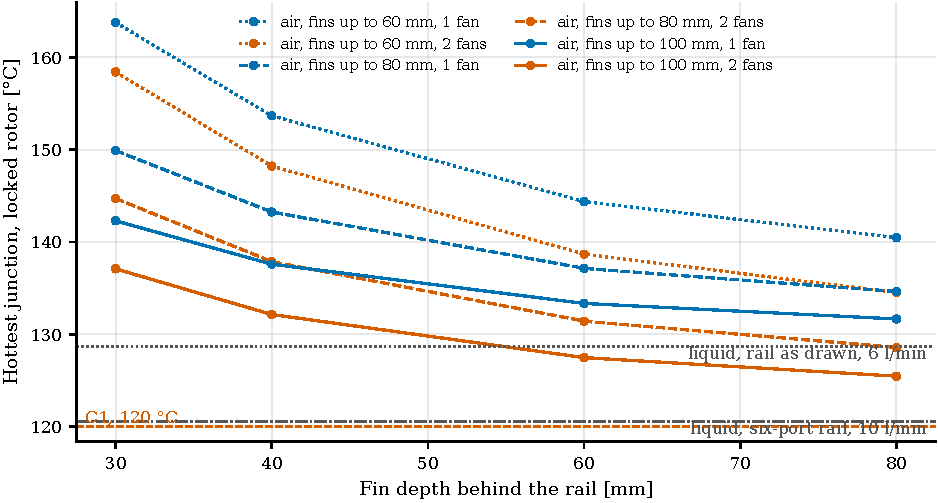
\includegraphics[width=\textwidth]{termica_raffreddamento_aria_liquido.pdf}
\caption{Forced air at \SI{50}{\celsius}: hottest junction at locked rotor
against the depth of fins attached behind the rail (\SI{20}{\milli\metre}
base, fins up to \SI{60}{}, \SI{80}{} or \SI{100}{\milli\metre} above the
board, one or two fans), with the two liquid rails for comparison;
pad \SI{0.50}{\celsius\per\watt}.}
\label{fig:coolair}
\end{figure}

\begin{figure}[htbp]
\centering
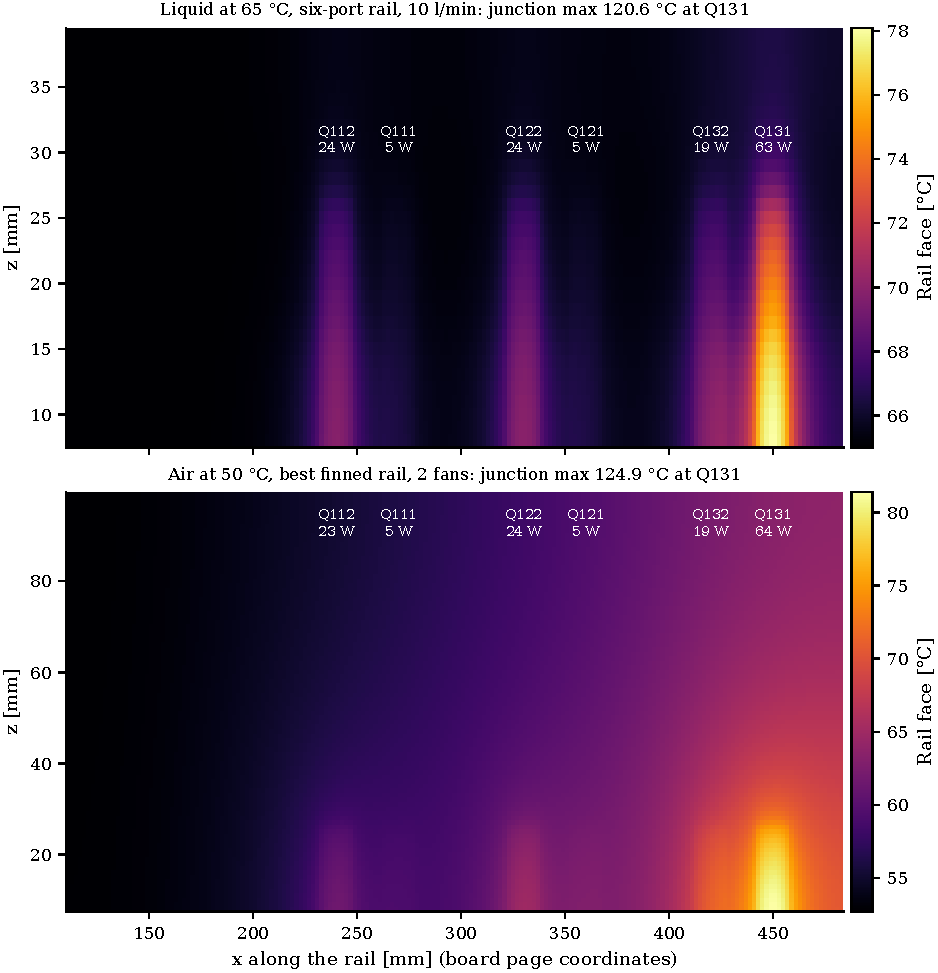
\includegraphics[width=\textwidth]{termica_raffreddamento_mappe.pdf}
\caption{Rail face temperature at locked rotor, peak current in leg~3.
Top: six-port liquid rail; the hottest strip is the lower part of the tab,
on the thin lip, farthest from the ports. Bottom: best forced-air sink; the
air warms along the rail.}
\label{fig:coolmaps}
\end{figure}

\subsection{The alternatives, on the same rail}
\label{sec:coolalt}

Between the die and the coolant there are four resistances: the die to the
case, the insulation, the spreading in the rail, the convection. At locked
rotor, on the six-port rail, the hottest device spends
\SI{14.4}{\celsius} in $\Rthjc$, \SI{31.6}{\celsius} in the pad and
\SI{9.6}{\celsius} between the rail face and the coolant. The pad is the
bottleneck, and it is the cheapest part to change. The pad itself
is a ceramic between two interfaces,
%
\begin{equation}
  \Rthcs = \frac{t_\mathrm{cer}}{k_\mathrm{cer} A} + \frac{2\,r_\mathrm{int}}{A},
\end{equation}
%
with $A = \SI{3.0}{\centi\metre\squared}$ for the tab. The
\SI{0.50}{\celsius\per\watt} of this chapter, with
\SI{0.63}{\milli\metre} alumina ($k = \SI{24}{\watt\per\metre\per\kelvin}$,
\SI{0.09}{\celsius\per\watt}), implies about
\SI{0.6}{\kelvin\centi\metre\squared\per\watt} per interface: a prudent
grease joint. A phase-change interface material under a specified clip
force reaches \SI{0.25}{\kelvin\centi\metre\squared\per\watt}, and aluminium
nitride ($k = \SI{170}{\watt\per\metre\per\kelvin}$) removes most of the
ceramic term. \Cref{tab:coolalt} runs every route on the same rail and loss
model.

\begin{table}[htbp]
\centering
\caption{Cooling alternatives on the six-port rail at \SI{10}{\litre\per\minute}
and \SI{65}{\celsius} (forced air at \SI{50}{\celsius} where stated). Worst
case: maximum $\Rthjc$, pad $+\SI{20}{\percent}$, maximum $\Rdson$, coolant
at \SI{70}{\celsius}, air at \SI{50}{\celsius}.}
\label{tab:coolalt}
\small
\begin{tabular}{lrrrr}
\toprule
 & $\Rthcs$ & Locked rotor & Worst case & With DPWM \\
Route (TO-247-4 unless stated) & [\si{\celsius\per\watt}] & [\si{\celsius}] & [\si{\celsius}] & [\si{\celsius}] \\
\midrule
Alumina, prudent value (as above) & 0.50 & 120.6 & 153.4 & 99.3 \\
Alumina + phase-change interface & 0.25 & 102.9 & 125.4 & 88.6 \\
\textbf{AlN + phase-change interface} & \textbf{0.18} & \textbf{97.9} & \textbf{117.8} & \textbf{85.6} \\
Copper spreader \SI{25\times 28}{\milli\metre} + AlN & 0.16 & 92.6 & 110.9 & 82.3 \\
Internally isolated, no external pad$^a$ & 0.08 & 98.3 & 116.7 & 85.8 \\
Forced air, one fan, AlN + phase change$^b$ & 0.18 & 108.3 & 129.1 & 85.0 \\
Top-side-cooled Q-DPAK, gap pad$^c$ & 0.61 & 139.4 & 179.9 & 110.3 \\
\bottomrule
\multicolumn{5}{l}{\footnotesize $^a$ internal ceramic counted as \SI{+0.10}{\celsius\per\watt} on $\Rthjc$; grease only outside.} \\
\multicolumn{5}{l}{\footnotesize $^b$ fins behind the rail, \SI{20}{\milli\metre} base, \SI{87\times 60}{\milli\metre} fins; coarse mesh.} \\
\multicolumn{5}{l}{\footnotesize $^c$ AIMCQ120R020M1T; $\Rthjc \approx \SI{0.26}{\celsius\per\watt}$ from its power rating; losses of the \device{} assumed.}
\end{tabular}
\end{table}

Route by route:
%
\begin{itemize}
  \item The interface decides more than the ceramic. Keeping
        alumina and changing only the interface material and the clamping
        gains \SI{17.7}{\celsius}; aluminium nitride adds \SI{5}{\celsius}
        more. The board does not change, the cost is a few euros, and the
        value becomes a mounting specification, confirmed by measuring the
        mounted pad.
  \item A copper spreader at drain potential between tab and pad
        spreads the flux over \SI{7}{\centi\metre\squared} and gains another
        \SI{5}{\celsius}. It is not worth it here: a second clamped joint,
        and spreaders of opposite potentials \SI{5}{\milli\metre} apart where the
        creepage asks for \SI{4.5}{}.
  \item Internally isolated TO-247-4 packages put the ceramic
        inside, under the die (Littelfuse ISO247, Navitas UHV-TO-247-4-ISO
        with AlN, Luminus ISOMOS~\cite{littelfuse_iso247,navitas_uhviso}):
        same footprint, no external pad, vendor claims of up to
        \SIrange{60}{64}{\percent} lower junction-to-heat-sink resistance. In
        this model they match the AlN pad, with one interface and one
        assembly step less. None is offered at
        \SI{16}{\milli\ohm} with AEC-Q101 qualification today, so it fails
        C4 and stays a production watch item.
  \item Top-side-cooled packages (Q-DPAK, TOLT, HU3PAK, U2) are now
        available in the automotive \SI{1200}{\volt} range down to
        \SI{19}{\milli\ohm}~\cite{infineon_aimcq}. Their top pad is the
        drain, about half the area of a TO-247 tab, and needs an insulating
        gap pad: thermally worse here, by \SI{19}{\celsius}. Their strengths are
        automated assembly and loop inductance, and adopting them would
        mean a new board.
  \item A plane on the bottom of the board does not help a through-hole
        device: only the drain lead is joined to the tab, and at
        \SI{18}{\celsius\per\watt} it carries at most \SI{4}{\percent} of the
        heat. A bottom-cooled SMD package needs eighty filled vias and an
        insulator under its drain pad, \SI{1.9}{\celsius\per\watt}, ten times
        the AlN pad.
  \item Classic heat sinks work only with the better pad and a fan,
        and then they work: one fan, \SI{108.3}{\celsius} at locked rotor and
        \SI{129.1}{\celsius} in the worst case. They lose on other
        grounds. The fins sit over the high-voltage board, so the
        enclosure must breathe outside air across it and the uncoated areas
        (terminals, connectors, test points) leave pollution degree~2; the
        fan is a wear part whose failure at standstill takes the junction
        towards the natural-convection figure within seconds, so it would
        need tachometer supervision and immediate derating; and the sink is
        about ten times the volume of the rail. The vehicle already has a
        liquid loop (\cref{tab:sysassume}).
\end{itemize}

\begin{finding}{Adopted cooling: six-port rail and aluminium nitride pad}
The adopted solution is the six-port liquid rail at \SI{10}{\litre\per\minute},
with \SI{0.63}{\milli\metre} aluminium nitride and a phase-change interface
on both faces under a specified clip force, $\Rthcs \le \SI{0.18}{\celsius\per\watt}$
as design value. The hottest junction at locked rotor falls from
\SI{120.6}{} to \SI{97.9}{\celsius}, the simultaneous worst case from
\SI{153.4}{} to \SI{117.8}{\celsius}: \SI{32.2}{\celsius} from the
\SI{150}{\celsius} limit, without touching the frozen board. The pad value
not to be exceeded at assembly becomes \SI{0.50}{\celsius\per\watt}, at which
C1 is still met on the real rail. The
device-level results of this chapter, computed on the ideal plate with the
prudent pad, remain a valid comparison between candidates; the absolute
temperatures of the design are those of \cref{tab:coolalt}.
\end{finding}

\section{Thermal transient}

The thermal time constant of the cold plate is of the order of seconds,
while the solver step is about \SI{1}{\micro\second} at \SI{20}{\kilo\hertz},
so a short window is simulated and an exponential identified from it. The
heat capacity of \SI{1000}{\joule\per\kelvin} is estimated from geometry: a
\SI{200}{}$\times$\SI{150}{}$\times$\SI{12}{\milli\metre} aluminium plate with
\SI{15}{\percent} of its volume taken by channels gives
\SI{744}{\joule\per\kelvin} of metal, \SI{204}{\joule\per\kelvin} of retained
coolant and roughly \SI{90}{\joule\per\kelvin} of fittings. The
identification gives $\tau = \SI{10.20}{\second}$ against
\SI{10.00}{\second} expected, and the temperature rise agrees with
$P_\mathrm{tot}\Rthha$ within \SI{1.6}{\percent}. The heat capacity affects
only the transient: all eleven steady-state operating points reproduce
bit-for-bit with the value doubled.

\section{The other components: temperature and life}
\label{sec:complife}

This section checks the other components of the power stage (the DC-link
films, the commutation ceramics and the shunts) against their manufacturers'
limits. Two assumptions frame it: the air inside the enclosure is
\SI{70}{\celsius} in normal operation and \SI{85}{\celsius} in a hot case,
since the liquid loop at \SI{65}{\celsius} sets the interior rather than the
\SI{50}{\celsius} outside; and the mission is \SI{8000}{\hour} of operation
with the bus energised, the usual order for fifteen years of a passenger car.

\begin{table}[htbp]
\centering
\caption{Stress, temperature and margin of the power-stage components that
carry high voltage or ripple current. Air inside the enclosure \SI{70}{\celsius},
hot case \SI{85}{\celsius}; power copper up to \SI{30}{\kelvin} above it
(\cref{tab:widths}).}
\label{tab:complife}
\small
\begin{tabularx}{\textwidth}{lllY}
\toprule
Component & Stress & Temperature & Margin \\
\midrule
Film C101, \SI{140}{\micro\farad} & \SI{13.7}{} of \SI{43.5}{\ampere}, \SI{0.37}{\watt} & hotspot $+\SI{1.5}{\kelvin}$ & \SI{63000}{\hour} at \SI{900}{\volt}, \SI{85}{\celsius} \\
Film C102, \SI{60}{\micro\farad} & \SI{5.9}{} of \SI{40}{\ampere}, \SI{0.09}{\watt} & hotspot $+\SI{0.6}{\kelvin}$ & as C101, slightly better \\
KC-LINK, $12\times\SI{47}{\nano\farad}$ & \SIrange{1.0}{2.0}{\ampere} each, \SI{2}{\mega\hertz} & a few tenths of a kelvin & \SI{12}{\ampere} allowed; C0G does not age \\
Shunts, \SI{0.5}{\milli\ohm} & \SI{0.45}{}/\SI{0.90}{\watt} rated/stalled & terminals \SIrange{100}{115}{\celsius} & \SIrange{5.0}{6.3}{\watt} allowed there \\
\bottomrule
\end{tabularx}
\end{table}

\paragraph{The film capacitors.} Their life is the only one in the table
that is consumed. The manufacturer gives it as a family of lines, life
against the ratio of operating to rated voltage, at
\SI{70}{}, \SI{85}{} and \SI{105}{\celsius}~\cite{vishay_mkp1848}; read from
the graph and interpolated in temperature, it gives \SI{94000}{\hour} at
rated voltage and \SI{70}{\celsius}, consistent with the
\SI{100000}{\hour} the datasheet declares, which is the check of the
reading. The self-heating is small, so life is a function of the air around
the capacitor (\cref{fig:filmlife}): the mission is met at \SI{900}{\volt}
continuous up to \SI{99.7}{\celsius} of air. The \SI{1100}{\volt} class
chosen for the voltage derating (\cref{sec:dclink}) is what buys this: at
the same temperature a \SI{900}{\volt} part would sit at its rated voltage.

\begin{figure}[htbp]
\centering
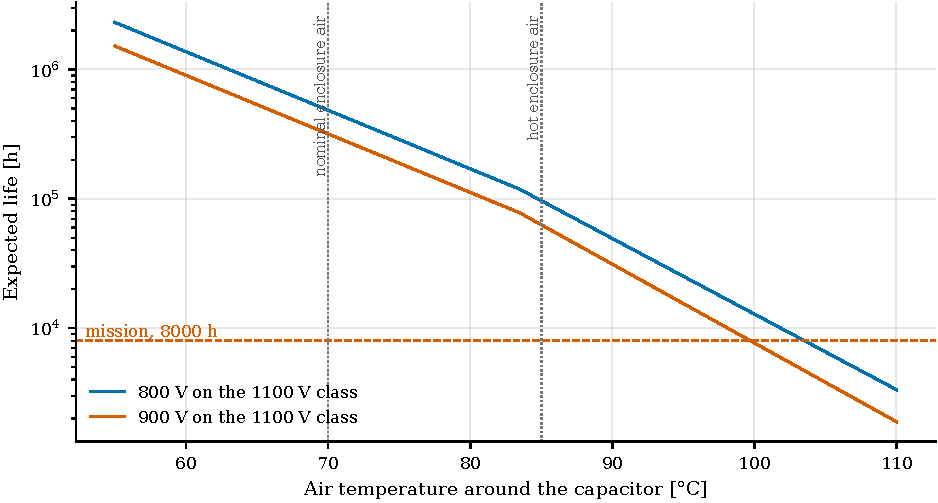
\includegraphics[width=\textwidth]{termica_componenti_vita_film.pdf}
\caption{Expected life of the DC-link film capacitors against the air
temperature around them, at the nominal and the maximum continuous bus
voltage, from the manufacturer's life curves.}
\label{fig:filmlife}
\end{figure}


\paragraph{The ceramics ring with the films.} At every switching edge the
step in bridge current is first supplied by the ceramics, then handed to
the films through their inductance, about \SI{11}{\nano\henry} with the
planes: a damped ring at
$f_0 = 1/(2\pi\sqrt{L\,C}) \approx \SI{2.0}{\mega\hertz}$ with
$C = \SI{564}{\nano\farad}$. With the energy of each ring
$\Delta I^2/(4\alpha)$, $\alpha = R/2L$, summed over six edges per switching
period, the ceramics carry \SIrange{12}{24}{\ampere} in total for a loop
resistance of \SIrange{4}{1}{\milli\ohm}: \SIrange{1}{2}{\ampere} each,
well inside their rating.

\paragraph{The shunts} dissipate a fifth of what their terminals allow even
in the hot case. What their temperature does affect is accuracy: with
\SI{100}{ppm\per\kelvin} including the copper terminals, a rise of
\SI{60}{\kelvin} above calibration is \SI{0.6}{\percent} of gain error, to be
added to the measurement budget or compensated with the cold-plate
thermistor.
